\documentclass[10pt,a4paper]{article}
\usepackage[margin=0.62in]{geometry}
\usepackage[T1]{fontenc}
\usepackage[utf8]{inputenc}
\usepackage{lmodern}
\usepackage{amsmath,amssymb}
\usepackage{booktabs}
\usepackage{tabularx}
\usepackage{array}
\usepackage{graphicx}
\usepackage{float}
\usepackage{subcaption}
\usepackage{enumitem}
\usepackage{xcolor}
\usepackage{hyperref}
\usepackage{microtype}
\usepackage{titlesec}
\usepackage{fancyhdr}
\usepackage[most]{tcolorbox}
\usepackage{tikz}
\usetikzlibrary{positioning,arrows.meta,calc,shapes.geometric,decorations.pathreplacing,fit}

\definecolor{brand}{HTML}{0D3B66}
\definecolor{accent}{HTML}{2A9D8F}
\definecolor{softbg}{HTML}{F4F8FB}
\definecolor{textdark}{HTML}{1E1E1E}

\hypersetup{
  colorlinks=true,
  linkcolor=brand,
  urlcolor=accent
}

\setlength{\parindent}{0pt}
\setlength{\parskip}{3pt}
\setlist[itemize]{leftmargin=1.2em,itemsep=1pt,topsep=2pt}

\titleformat{\section}{\color{brand}\large\bfseries}{\thesection.}{0.4em}{}
\titleformat{\subsection}{\color{textdark}\bfseries}{\thesubsection}{0.4em}{}
\titlespacing*{\section}{0pt}{8pt}{4pt}
\titlespacing*{\subsection}{0pt}{6pt}{3pt}

\pagestyle{fancy}
\fancyhf{}
\fancyhead[L]{\small CS671 Technical Model Report}
\fancyhead[R]{\small Paired Diffusion (Brain)}
\fancyfoot[C]{\small \thepage}
\setlength{\headheight}{14pt}

\begin{document}

% -------------------- Header Block --------------------
\begin{tcolorbox}[
  enhanced,
  colback=softbg,
  colframe=brand,
  boxrule=0.9pt,
  arc=2mm,
  left=5pt,right=5pt,top=5pt,bottom=5pt
]
\centering
{\Large\bfseries\color{brand} CS671 -- Deep Learning and Its Applications}\\[2pt]
{\large\bfseries Technical Documentation Report}\\[6pt]
{\normalsize\bfseries Model: Paired Diffusion (Brain)}\\[4pt]
\small
Project Group: 5 \quad Region: Brain \quad Modality: Paired (CT $\to$ MRI)
\end{tcolorbox}

\section{ARCHITECTURAL OVERVIEW}
Paired Diffusion utilizes a Latent Diffusion Model (LDM) framework to perform CT-to-MRI synthesis. Unlike GAN-based approaches, diffusion models learn the data distribution by reversing a gradual denoising process. In this implementation, the model is conditioned on CT features to guide the generation of aligned MRI slices in a compressed latent space.

\subsection{Latent Diffusion Architecture}
The implementation utilizes a high-fidelity Latent Diffusion Model (LDM) where denoising occurs in a compressed $64 \times 64 \times 4$ latent space. A critical architectural enhancement in this project is the modification of the Variational Autoencoder (VAE) to include custom skip-connections for spatial preservation.

\begin{figure}[H]
\centering
\resizebox{\textwidth}{!}{
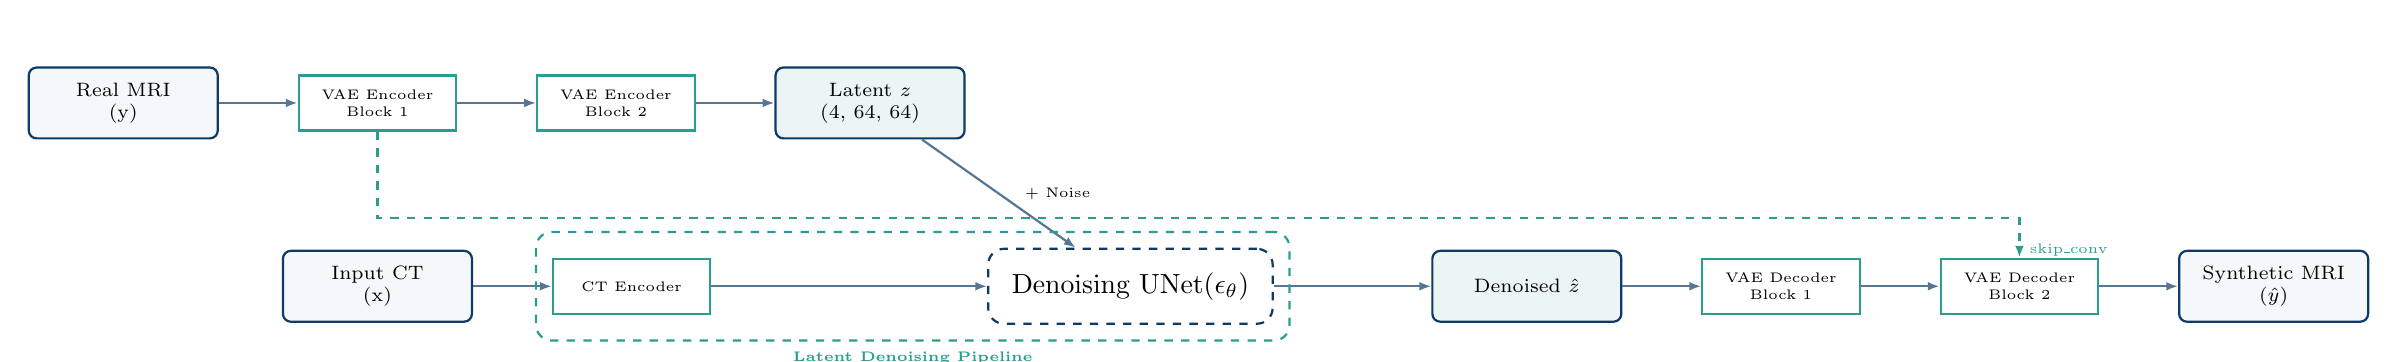
\begin{tikzpicture}[
    node distance=5mm and 10mm,
    block/.style={draw=brand, thick, fill=softbg, minimum width=2.4cm, minimum height=0.9cm, align=center, rounded corners=1mm, font=\scriptsize},
    module/.style={draw=accent, thick, fill=white, minimum width=2.0cm, minimum height=0.7cm, align=center, font=\tiny},
    arr/.style={-{Latex[length=1.5mm]}, thick, draw=brand!70},
    skip/.style={-{Latex[length=1.5mm]}, thick, dashed, draw=accent}
]
    % VAE Encoder Path
    \node[block] (in_mri) {Real MRI\\(y)};
    \node[module, right=of in_mri] (enc_1) {VAE Encoder\\Block 1};
    \node[module, right=of enc_1] (enc_2) {VAE Encoder\\Block 2};
    \node[block, right=of enc_2, fill=accent!10] (latent) {Latent $z$\\ (4, 64, 64)};

    % Denoising Path (Middle)
    \node[block, below=1.5cm of enc_1] (ct_in) {Input CT\\(x)};
    \node[module, right=of ct_in] (ct_enc) {CT Encoder};
    \node[draw=brand, thick, dashed, rounded corners=2mm, inner sep=3mm, right=3.5cm of ct_enc] (unet) {Denoising UNet\\($\epsilon_\theta$)};
    
    % VAE Decoder Path (Bottom)
    \node[block, right=2.0cm of unet, fill=accent!10] (z_hat) {Denoised $\hat{z}$};
    \node[module, right=of z_hat] (dec_1) {VAE Decoder\\Block 1};
    \node[module, right=of dec_1] (dec_2) {VAE Decoder\\Block 2};
    \node[block, right=of dec_2] (out_mri) {Synthetic MRI\\($\hat{y}$)};

    % Connections
    \draw[arr] (in_mri) -- (enc_1); \draw[arr] (enc_1) -- (enc_2); \draw[arr] (enc_2) -- (latent);
    \draw[arr] (latent) -- (unet) node[midway, right=2mm, font=\tiny] {+ Noise};
    \draw[arr] (ct_in) -- (ct_enc);
    \draw[arr] (ct_enc) -- (unet);
    \draw[arr] (unet) -- (z_hat);
    \draw[arr] (z_hat) -- (dec_1); \draw[arr] (dec_1) -- (dec_2); \draw[arr] (dec_2) -- (out_mri);

    % Skip Connections
    \draw[skip] (enc_1.south) |- ($(dec_2.north) + (0,0.5)$) -- (dec_2.north) node[pos=0.8, right, font=\tiny, color=accent] {skip\_conv};
    
    % Grouping
    \node[draw=accent, dashed, thick, rounded corners=2mm, inner sep=2mm, fit=(ct_enc) (unet), label={[font=\tiny\bfseries, color=accent]below:Latent Denoising Pipeline}] (group) {};
\end{tikzpicture}
}
\caption{Enhanced Latent Diffusion Architecture: The implementation features a modified VAE where intermediate encoder activations are projected via $1 \times 1$ convolutions and injected into the decoder, significantly improving anatomical registration.}
\end{figure}

\textbf{VAE Skip-Connection Injection:} 
A key implementation detail in the \texttt{VAEDecode} class is the manual injection of encoder activations into the upsampling blocks. We override the standard forward pass to capture features from the \texttt{down\_blocks} and project them using four learned $1 \times 1$ convolution layers (\texttt{skip\_conv\_1} to \texttt{skip\_conv\_4}). These weights are initialized to $1e-5$ to maintain stability while allowing the model to recover high-resolution structural information that is typically lost during VAE compression.

\textbf{LoRA Adaptation for UNet and VAE:} 
To adapt the pre-trained diffusion models to medical imagery without catastrophic forgetting, we utilize Low-Rank Adaptation (LoRA). The implementation targets all linear and convolutional layers in both the UNet (denoiser) and the VAE (autoencoder), including \texttt{to\_q}, \texttt{to\_k}, \texttt{to\_v}, and \texttt{proj\_out} modules. This allows for parameter-efficient fine-tuning of the complex CT-to-MRI intensity mapping while keeping the backbone frozen.

\textbf{Conditioning Mechanism (Cross-Attention):} 
The UNet2DConditionModel incorporates the CT conditioning through spatial cross-attention layers. CT features are projected into the UNet's latent space, where they act as the "key" and "value" pairs, guiding the denoising of the Gaussian noise into a structurally consistent MRI representation.

\section{TRAINING WORKFLOW}
Training involves a forward diffusion process (adding noise) and a learned reverse process (denoising).

\begin{figure}[H]
\centering
\resizebox{0.8\textwidth}{!}{
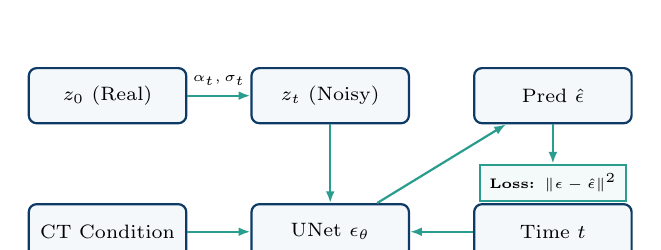
\begin{tikzpicture}[
    node distance=8mm,
    box/.style={draw=brand, thick, fill=softbg, minimum width=2cm, minimum height=0.7cm, align=center, rounded corners=1mm, font=\scriptsize},
    arr/.style={-{Latex[length=1.5mm]}, thick, draw=accent}
]
    \node[box] (z0) {$z_0$ (Real)};
    \node[box, right=of z0] (zt) {$z_t$ (Noisy)};
    \node[box, right=of zt] (pred) {Pred $\hat{\epsilon}$};
    \node[box, below=1cm of zt] (unet) {UNet $\epsilon_\theta$};
    \node[box, left=of unet] (ct) {CT Condition};
    \node[box, right=of unet] (time) {Time $t$};

    \draw[arr] (z0) -- (zt) node[midway, above, font=\tiny] {$\alpha_t, \sigma_t$};
    \draw[arr] (zt) -- (unet);
    \draw[arr] (ct) -- (unet);
    \draw[arr] (time) -- (unet);
    \draw[arr] (unet) -- (pred);
    
    \node[draw=accent, thick, fill=accent!5, below=5mm of pred, font=\tiny\bfseries] (loss) {Loss: $\|\epsilon - \hat{\epsilon}\|^2$};
    \draw[arr] (pred) -- (loss);
\end{tikzpicture}
}
\caption{Forward and Reverse Diffusion: Learning to denoise conditioned on CT and Time.}
\end{figure}

\textbf{Objective Function and Sampler Dynamics:} 
The implementation utilizes a standard diffusion objective, minimizing the Mean Squared Error (MSE) between the added Gaussian noise $\epsilon$ and the network's prediction $\epsilon_\theta(z_t, t, x)$. For efficient inference, we employ a \texttt{DDPMScheduler} with custom timestep spacing. The sampling trajectory is deterministic, ensuring that for a given CT input, the model produces a consistent MRI reconstruction.

\section{INFERENCE PIPELINE}
Inference (sampling) is an iterative process where the model starts from random noise and gradually removes it to reveal the synthetic MRI.

\begin{figure}[H]
\centering
\resizebox{0.9\textwidth}{!}{
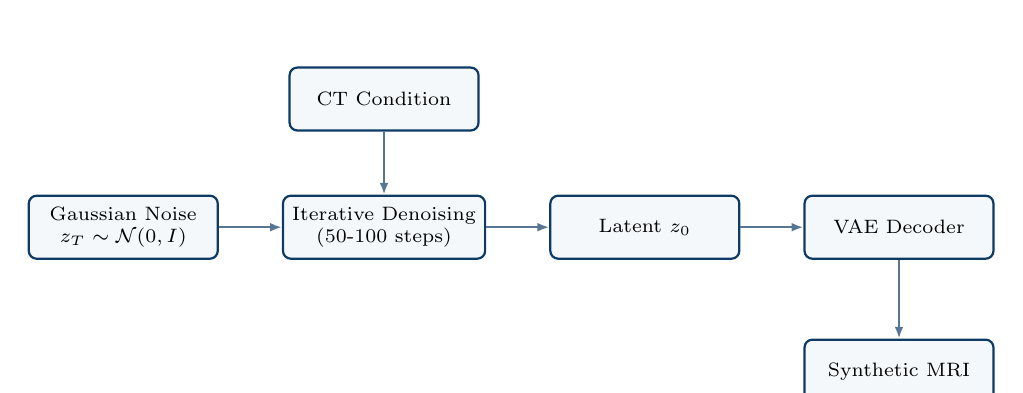
\begin{tikzpicture}[
    node distance=8mm,
    block/.style={draw=brand, thick, fill=softbg, minimum width=2.4cm, minimum height=0.8cm, align=center, rounded corners=1mm, font=\scriptsize},
    arr/.style={-{Latex[length=1.5mm]}, thick, draw=brand!70}
]
    \node[block] (noise) {Gaussian Noise\\$z_T \sim \mathcal{N}(0, I)$};
    \node[block, right=of noise] (loop) {Iterative Denoising\\(50-100 steps)};
    \node[block, right=of loop] (z0) {Latent $z_0$};
    \node[block, right=of z0] (dec) {VAE Decoder};
    \node[block, below=1cm of dec] (out) {Synthetic MRI};

    \draw[arr] (noise) -- (loop);
    \draw[arr] (loop) -- (z0);
    \draw[arr] (z0) -- (dec);
    \draw[arr] (dec) -- (out);

    \node[block, above=8mm of loop] (ct) {CT Condition};
    \draw[arr] (ct) -- (loop);
\end{tikzpicture}
}
\caption{Inference Sampling: Iterative reconstruction guided by CT conditioning.}
\end{figure}

During inference, we use schedulers like DDIM or PNDM to accelerate the sampling process. The input CT volume is encoded once, and its features are used as constant conditioning throughout the denoising iterations. This ensures that every generated MRI slice is perfectly aligned with the anatomical structures present in the CT.

\end{document}
